% definitions of long commands and graphical objects 

\definecolor{glossary-link-color}{RGB}{129, 19, 49}
\definecolor{revision-color}{RGB}{100,0,0}

% \makeatletter
% \newcommand*{\glsplainhyperlink}[2]{%
%     \colorlet{currenttext}{.}% store current text color
%     \colorlet{currentlink}{\@linkcolor}% store current link color
%     \hypersetup{linkcolor=glossary-link-color}% set link color
%     \hyperlink{#1}{#2}%
%     \hypersetup{linkcolor=currentlink}% reset to default
% }
% \let\@glslink\glsplainhyperlink
% \makeatother

% Define a new command that draws a square without vertical sides:
%  boundary for a one-dimensional line manifold
\providecommand{\mlineeq}{{\mathord{%
                \tikz[baseline=-0.1ex]{
                    \tikzmath{\size = 0.06ex;  }
                    \draw[line width=1pt, draw opacity =1] (0,0) -- (\size,0);
                }%
            }}}
% in boundary for a one-dimensional line manifold
\providecommand{\mlineineq}{{\mathord{%
                \tikz[baseline=-0.1ex]{

                    \tikzmath{\size = 0.06ex;  }
                    \draw[line width=1pt, draw opacity =0.5] (0,0) -- (\size,0);
                    \filldraw[color=black, fill=black](0,0) circle (0.05);
                }
            }}}

% out boundary for a one-dimensional line manifold
\providecommand{\mlineouteq}{{\mathord{%
                \tikz[baseline=-0.1ex]{

                    \tikzmath{\size = 0.06ex;  }
                    \draw[line width=1pt, draw opacity =0.5] (0,0) -- (\size,0);
                    \filldraw[color=black, fill=black](\size,0) circle (0.05);
                }
            }}}

\providecommand{\mwalleq}{{\mathord{%
                \tikz[baseline=-0.1ex]{

                    \tikzmath{\size = 0.03ex;  }

                    \draw[line width=1pt] (0,0) -- (\size,0);
                    \draw[line width=1pt, draw opacity = 0.15] (\size,0) -- (\size,\size);
                    \draw[line width=1pt] (\size,\size) -- (0,\size);
                    \draw[line width=1pt, draw opacity = 0.15] (0,\size) -- (0,0);
                }%
            }}}

\providecommand{\mtopeq}{{\mathord{%
                \tikz[baseline=-0.1ex]{

                    \tikzmath{\size = 0.03ex;  }

                    \draw[line width=1pt, draw opacity = 0.15] (0,0) -- (\size,0);
                    \draw[line width=1pt, draw opacity = 0.15] (\size,0) -- (\size,\size);
                    \draw[line width=1pt] (\size,\size) -- (0,\size);
                    \draw[line width=1pt, draw opacity = 0.15] (0,\size) -- (0,0);
                }%
            }}}
\providecommand{\mbottomeq}{{\mathord{%
                \tikz[baseline=-0.1ex]{

                    \tikzmath{\size = 0.03ex;  }

                    \draw[line width=1pt] (0,0) -- (\size,0);
                    \draw[line width=1pt, draw opacity = 0.15] (\size,0) -- (\size,\size);
                    \draw[line width=1pt, draw opacity = 0.15] (\size,\size) -- (0,\size);
                    \draw[line width=1pt, draw opacity = 0.15] (0,\size) -- (0,0);
                }%
            }}}


% symbol for the bottom - left vertex of a square

\providecommand{\mleftbottomeq}{{\mathord{%
                \tikz[baseline=-0.1ex]{

                    \tikzmath{\size = 0.03ex;  }

                    \draw[line width=1pt, draw opacity = 0.15] (0,0) -- (\size,0);
                    \draw[line width=1pt, draw opacity = 0.15] (\size,0) -- (\size,\size);
                    \draw[line width=1pt, draw opacity = 0.15] (\size,\size) -- (0,\size);
                    \draw[line width=1pt, draw opacity = 0.15] (0,\size) -- (0,0);

                    \filldraw[color=black, fill=black](0,0) circle (0.04);

                }%
            }}}

\providecommand{\myineq}{{\mathord{%
                \tikz[baseline=-0.1ex]{

                    \tikzmath{\size = 0.03ex;  }


                    \draw[line width=1pt, draw opacity = 0.15] (0,0) -- (\size,0);
                    \draw[line width=1pt, draw opacity = 0.15] (\size,0) -- (\size,\size);
                    \draw[line width=1pt, draw opacity = 0.15] (\size,\size) -- (0,\size);
                    \draw[line width=1pt] (0,\size) -- (0,0);
                }%
            }}}

\providecommand{\myinwalleq}{{\mathord{%
                \tikz[baseline=-0.1ex]{

                    \tikzmath{\size = 0.03ex;  }


                    \draw[line width=1pt] (0,0) -- (\size,0);
                    \draw[line width=1pt, draw opacity = 0.15] (\size,0) -- (\size,\size);
                    \draw[line width=1pt] (\size,\size) -- (0,\size);
                    \draw[line width=1pt] (0,\size) -- (0,0);
                }%
            }}}

\providecommand{\myouteq}{{\mathord{%
                \tikz[baseline=-0.1ex]{

                    \tikzmath{\size = 0.03ex;  }

                    \draw[line width=1pt, draw opacity = 0.15] (0,0) -- (\size,0);
                    \draw[line width=1pt] (\size,0) -- (\size,\size);
                    \draw[line width=1pt, draw opacity = 0.15] (\size,\size) -- (0,\size);
                    \draw[line width=1pt, draw opacity = 0.15] (0,\size) -- (0,0);
                }%
            }}}

\providecommand{\msquareeq}{{\mathord{%
                \tikz[baseline=-0.1ex]{

                    \tikzmath{\size = 0.03ex;  }


                    \draw[line width=1pt] (0,0) -- (\size,0);
                    \draw[line width=1pt] (\size,0) -- (\size,\size);
                    \draw[line width=1pt] (\size,\size) -- (0ex,\size);
                    \draw[line width=1pt] (0ex,\size) -- (0ex,0ex);
                }%
            }}}

\providecommand{\mcirceq}{{\mathord{%
                \tikz[baseline=-0.1ex]{
                    \draw[line width=1pt] (0,0) circle [radius=0.5ex];
                }%
            }}}

\providecommand{\mellipseeq}{{\mathord{%
                \tikz[baseline=-0.3ex]{
                    \draw[line width=0.8pt] (0,0) ellipse [x radius=0.6ex, y radius=0.3ex];
                }%
            }}}

\providecommand{\mcircineq}{{\mathord{%
                \tikz[baseline=-0.5ex]{
                    \draw[line width=1pt] (0,0) circle [radius=0.3ex];
                    \draw[line width=1pt, draw opacity = 0.15] (0,0) circle [radius=.7ex];
                }%
            }}}

\providecommand{\mcircouteq}{{\mathord{%
                \tikz[baseline=-0.5ex]{
                    \draw[line width=1pt, draw opacity = 0.15] (0,0) circle [radius=0.3ex];
                    \draw[line width=1pt] (0,0) circle [radius=.65ex];
                }%
            }}}

\providecommand{\libtickzpicture}{
    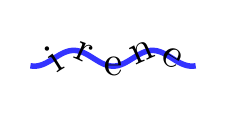
\begin{tikzpicture}[scale=1, baseline={(current bounding box.center)}]
        \def\s{80}
        \def\A{0.1}
        \def\xmax{1.5}
        \def\scalefactorletters{1.5}
        \def\radtodeg{360.0/(2.0*pi)}
        \def\degtorad{1.0/(360.0/(2.0*pi))}

        \draw[color={rgb,255:red,0; green,0; blue,255}, opacity=0.8, line width=2pt] plot[domain=-0.2:1.2, samples=100]
        (\x*\xmax, {\A*sin(2*pi*\x*\xmax*\radtodeg)});

        \node at (0*\xmax, {\A*sin(2*pi* 0*\xmax * \radtodeg)})
        [rotate= atan(\A *2*pi  * cos(2*pi * 0*\xmax * \radtodeg))] {\scalebox{\scalefactorletters}{i}};
        \node at (0.25*\xmax, {\A*sin(2*pi* 0.25*\xmax * \radtodeg)})
        [rotate= atan(\A *2*pi  * cos(2*pi * 0.25*\xmax * \radtodeg))] {\scalebox{\scalefactorletters}{r}};
        \node at (0.5*\xmax, {\A*sin(2*pi* 0.5*\xmax * \radtodeg)})
        [rotate= atan(\A *2*pi  * cos(2*pi * 0.5*\xmax * \radtodeg))] {\scalebox{\scalefactorletters}{e}};
        \node at (0.75*\xmax, {\A*sin(2*pi* 0.75*\xmax * \radtodeg)})
        [rotate= atan(\A *2*pi  * cos(2*pi * 0.75*\xmax * \radtodeg))] {\scalebox{\scalefactorletters}{n}};
        \node at (1.0*\xmax, {\A*sin(2*pi* 1.0*\xmax * \radtodeg)})
        [rotate= atan(\A *2*pi  * cos(2*pi * 1.00*\xmax * \radtodeg))] {\scalebox{\scalefactorletters}{e}};
    \end{tikzpicture}%
}

\DeclareRobustCommand{\libsymbol}{%
    \raisebox{0.8ex}{%
        \scalebox{0.55}{\libtickzpicture}
        \vspace{-.5cm}
        \hspace{-0.2cm}
    }
}

\DeclareRobustCommand{\libsymbolfortitle}{%
    \raisebox{0.4ex}{%
        \scalebox{1.5}{
            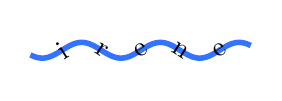
\begin{tikzpicture}[scale=1, baseline={(current bounding box.center)}]
                \def\s{80}
                \def\A{0.1}
                \def\xmax{2}
                \def\scalefactorletters{1}
                \def\radtodeg{360.0/(2.0*pi)}
                \def\degtorad{1.0/(360.0/(2.0*pi))}

                \draw[color={rgb,255:red,0; green,80; blue,255}, opacity=0.8, line width=2pt] plot[domain=-0.2:1.2, samples=100]
                (\x*\xmax, {\A*sin(2*pi*\x*\xmax*\radtodeg)});

                \node at (0*\xmax, {\A*sin(2*pi* 0*\xmax * \radtodeg)})
                [rotate= atan(\A *2*pi  * cos(2*pi * 0*\xmax * \radtodeg))] {\scalebox{\scalefactorletters}{i}};
                \node at (0.25*\xmax, {\A*sin(2*pi* 0.25*\xmax * \radtodeg)})
                [rotate= atan(\A *2*pi  * cos(2*pi * 0.25*\xmax * \radtodeg))] {\scalebox{\scalefactorletters}{r}};
                \node at (0.5*\xmax, {\A*sin(2*pi* 0.5*\xmax * \radtodeg)})
                [rotate= atan(\A *2*pi  * cos(2*pi * 0.5*\xmax * \radtodeg))] {\scalebox{\scalefactorletters}{e}};
                \node at (0.75*\xmax, {\A*sin(2*pi* 0.75*\xmax * \radtodeg)})
                [rotate= atan(\A *2*pi  * cos(2*pi * 0.75*\xmax * \radtodeg))] {\scalebox{\scalefactorletters}{n}};
                \node at (1.0*\xmax, {\A*sin(2*pi* 1.0*\xmax * \radtodeg)})
                [rotate= atan(\A *2*pi  * cos(2*pi * 1.00*\xmax * \radtodeg))] {\scalebox{\scalefactorletters}{e}};
            \end{tikzpicture}%
            % }
        }%
        \vspace{-.1cm}
        % \hspace{-0.2cm}
    }
}




% define \libname in such a way that it can be rendered in Section titles too: \libnameforsectiontitle
\newsavebox{\libnamebox}

\AtBeginDocument{%
    \sbox{\libnamebox}{%
        \raisebox{1.0ex}{%
            \scalebox{0.8}{\libtickzpicture}
        }%
    }%
}

\DeclareRobustCommand{\libsymbolforsectiontitle}{\usebox{\libnamebox}}
\newcommand{\libnameforsectiontitle}{\texorpdfstring{\libsymbolforsectiontitle}{IRENE}}



\providecommand{\mtitlecover}{IRENE: A fluId layeR finite-Element softwarE}

\providecommand{\be}{\begin{equation}}
        \providecommand{\ee}{\end{equation}}
\providecommand{\bsp}{\begin{split}}
        \providecommand{\esp}{\end{split}}
\providecommand{\bea}{\begin{eqnarray}}
        \providecommand{\eea}{\end{eqnarray}}
\providecommand{\beas}{\begin{eqnarray*}}
        \providecommand{\eeas}{\end{eqnarray*}}
\providecommand{\msquareeqcap}{{\protect \msquareeq}}
\providecommand{\myineqcap}{{\protect \myineq}}
\providecommand{\vmyin}{$v_\myineqcap$}
\providecommand{\diffgeosample}{\begin{align}\nn\nabla_i v^j                    & = \\ \nn
             \partial_i v^j + \Gamma^i_{jk} v^k &\end{align}}
\providecommand{\diffgeotext}{$\text{Differential geometry}$}
\providecommand{\pomsqeqcap}{{\protect \pomsqeq}}
\providecommand{\pomcirceqcap}{{\protect \pomcirceq}}
\providecommand{\mcirceqcap}{{\protect \mcirceq}}
\providecommand{\mellipseeqcap}{{\protect \mellipseeq}}
\providecommand{\mtlefteqcap}{{\protect \mtlefteq}}
\providecommand{\mtopeqcap}{{\protect \mtopeq}}
\providecommand{\mbottomeqcap}{{\protect \mbottomeq}}
\providecommand{\mleftbottomeqcap}{{\protect \mleftbottomeq}}
\providecommand{\sigmaast}{{\sigma^{\ast}}}
\providecommand{\vbar}{\overline{v}}
\providecommand{\bvbar}{{\bm \vbar}}
\providecommand{\wbar}{\overline{w}}
\providecommand{\testfunc}[1]{{\nu_{#1}}}
% vector tangent to the coordinate line in a differential manifold
\providecommand{\evec}[2]{{e_{#1}^{#2}}}
\providecommand{\bevec}[1]{{{\bm e}_{#1}}}
\providecommand{\titleditem}[2]{\item \textbf{#1.} \protect#2}
\providecommand{\mcircineqcap}{{\protect \mcircineq}}
\providecommand{\mcircouteqcap}{{\protect \mcircouteq}}
\providecommand{\om}{\Omega}
\providecommand{\omc}{\Omega^\current}
\providecommand{\omr}{\Omega^\reference}
\providecommand{\pom}{{\partial \om}}
\providecommand{\pom}{{\partial \om}}
\providecommand{\pomsqeq}{\pom_\msquareeq}
\providecommand{\pomineq}{\pom_\myineqcap}
\providecommand{\pominc}{$\pomineqc$}
\providecommand{\pomsqc}{$\pomsqeqc$}
\providecommand{\pomsqr}{$\pomsqeqr$}
\providecommand{\current}{\textrm{c}}
\providecommand{\reference}{\textrm{r}}
\providecommand{\pomsqeqc}{\pom_\msquareeq^{\current}}
\providecommand{\pomsqeqr}{\pom_\msquareeq^{\reference}}
\providecommand{\pomineqc}{\pom_\myineqcap^{\current}}
\providecommand{\pomineqr}{\pom_\myineqcap^{\reference}}
\providecommand{\pomin}{$\pomineq$}
\providecommand{\pomout}{$\pomouteq$}
\providecommand{\pomouteq}{\pom_\myouteqcap}
\providecommand{\pomouteqc}{\pom_\myouteqcap^{\current}}
\providecommand{\pomouteqr}{\pom_\myouteqcap^{\reference}}
\providecommand{\pominwalleq}{\pom_\myinwalleqcap}
\providecommand{\pomcirceq}{{\pom_\mcirceqcap}}
\providecommand{\pomcircone}{$\pomcirceqone$}
\providecommand{\pomcirctwo}{$\pomcirceqtwo$}
\providecommand{\pomcirceqone}{{\pom_{\mcirceqcap 1}}}
\providecommand{\pomcirceqtwo}{{\pom_{\mcirceqcap 2}}}
\providecommand{\pomellipseeqc}{{\pom_\mellipseeqcap^{\current}}}
\providecommand{\pomellipsec}{$\pomellipseeqc\;$}
\providecommand{\pomellipser}{$\pomellipseeqr\;$}
\providecommand{\pomellipseeqr}{{\pom_\mellipseeqcap^{\reference}}}
\providecommand{\pomcirc}{$\pomcirceq$}
\providecommand{\pomoutc}{$\pomouteqc\;$}
\providecommand{\nmhalf}{{n-1/2}}
\providecommand{\nmthalf}{{n-3/2}}
\providecommand{\nmthreehalf}{{n-3/2}}
\providecommand{\fn}[2]{{#1}^{#2}}
\providecommand{\fni}[3]{{#1}^{#2,\,#3}}
\providecommand{\fnij}[4]{{#1}^{#2,\,#3 }_{\phantom{#2,\,} #4}}
\providecommand{\pomcircin}{$\pom_\mcircineqcap$}
\providecommand{\pomcircout}{$\pom_\mcircouteqcap$}
\providecommand{\pomcircineq}{\pom_\mcircineqcap}
\providecommand{\pomweq}{\pom_\mwalleqcap}
\providecommand{\pomlineeq}{\pom_\mlineeqcap}
\providecommand{\omlineeq}{\om_\mlineeqcap}
\providecommand{\omlineeqr}{\om_\mlineeqcap^\reference}
\providecommand{\omlineeqc}{\om_\mlineeqcap^\current}
\providecommand{\pomline}{$\pom_\mlineeqcap$}
\providecommand{\pomlineineq}{\pom_\mlineineqcap}
\providecommand{\pomlinein}{$\pom_\mlineineqcap$}
\providecommand{\pomlineouteq}{\pom_\mlineouteqcap}
\providecommand{\pomlineout}{$\pom_\mlineouteqcap$}
\providecommand{\pomw}{$\pom_\mwalleq$}
\providecommand{\mwalleqcap}{{\protect \mwalleq}}
\providecommand{\mlineeqcap}{{\protect \mlineeq}}
\providecommand{\mlineineqcap}{{\protect \mlineineq}}
\providecommand{\mlineouteqcap}{{\protect \mlineouteq}}

% reference and current boundaries 
\providecommand{\pomcircineqc}{\pomcircineq^\current}
\providecommand{\pomlineeqc}{\pomlineeq^\current}
\providecommand{\pomlineeqr}{\pomlineeq^\reference}
\providecommand{\pomlineineqc}{\pomlineineq^\current}
\providecommand{\pomlineineqr}{\pomlineineq^\reference}
\providecommand{\pomcircineqr}{\pomcircineq^\reference}
\providecommand{\pomlineouteqr}{\pomlineouteq^\reference}
\providecommand{\pomlineouteqc}{\pomlineouteq^\current}
\providecommand{\pomcircouteqc}{\pomcircouteq^\current}
\providecommand{\pomcircouteq}{\pom_\mcircouteqcap}
\providecommand{\pomcircouteqc}{\pomcircouteq^\current}
\providecommand{\pomcircouteqr}{\pomcircouteq^\reference}
\providecommand{\pomweqc}{\pomweq^{\current}}
\providecommand{\pomweqr}{\pomweq^{\reference}}
\providecommand{\pomwc}{$\pomweqc$}
\providecommand{\pomwr}{$\pomweqr$}


\providecommand{\fetatan}{{f_\eta}}
\providecommand{\fetanorm}{{\textswab{f}_\eta}}
\providecommand{\fkap}{{f_\kap}}
\providecommand{\pomtopeq}{\pom_\mtopeqcap}

\providecommand{\pomtopeqc}{\pom_\mtopeqcap^{\current}}
\providecommand{\pomtopc}{$\pomtopeqc$}
\providecommand{\pombottomc}{$\pombottomeqc$}

\providecommand{\pomtopbottomc}{$\pomtopeqc \cup \pombottomeqc$}



\providecommand{\pomlefteqr}{\pom_\mlefteqcap^{\reference}}
\providecommand{\pomtopeqr}{\pom_\mtopeqcap^{\reference}}
\providecommand{\pombottomeq}{\pom_\mbottomeqcap}
\providecommand{\pombottomeqc}{\pom_\mbottomeqcap^{\current}}
\providecommand{\pomleftbottomeqc}{\pom_\mleftbottomeqcap^{\current}}
\providecommand{\pombottomeqr}{\pom_\mbottomeqcap^{\reference}}
\providecommand{\pomleftbottomeqr}{\pom_\mleftbottomeqcap^{\reference}}
\providecommand{\pombottom}{$\pombottomeq$}
\providecommand{\pomsq}{$\pomsqeq$}
\providecommand{\manifold}{\mathscr{M}}

% length elements in reference and current configurations
\providecommand{\lr}{l_{\reference}}
\providecommand{\lc}{l_{\current}}


\providecommand{\fluid}{\mathrm{\scalebox{0.6}{F}}}
\providecommand{\bod}{\mathrm{\scalebox{0.6}{B}}}
\providecommand{\ela}{\mathrm{\scalebox{0.6}{E}}}
\providecommand{\mem}{\mathrm{\scalebox{0.6}{M}}}
\providecommand{\dom}{\mathrm{\scalebox{0.6}{D}}}

\providecommand{\lapl}{\mathrm{\scalebox{0.6}{L}}}


\providecommand{\pomtop}{$\pomtopeq$}
\providecommand{\nomega}{\psi}
\providecommand{\nablz}{\phi}
\providecommand{\centerr}{{\bf c}}
\providecommand{\kap}{\kappa}
\providecommand{\nab}{\nabla}
\providecommand{\newt}{\text{N}}
\providecommand{\kb}{k_{\text B}}
\providecommand{\mic}{\mu \met}
\providecommand{\mm}{\text{mm}}
\providecommand{\km}{\text{Km}}
\providecommand{\rad}{\text{rad}}
\providecommand{\pas}{\text{Pa}}
\providecommand{\met}{\text{m}}
\providecommand{\newt}{\text{N}}
\providecommand{\kg}{\text{kg}}
\providecommand{\gr}{\text{g}}
\providecommand{\nsteps}{N_{\text s}}
\providecommand{\minute}{\text{min}}
\providecommand{\hour}{\text{hr}}
\providecommand{\Om}{\Omega}
% do not call this `\sec', it would conflict with secant definition build into latex
\providecommand{\second}{\text{s}}
\providecommand{\msecond}{\text{ms}}
\providecommand{\kel}{K}
\providecommand{\bx}{{\boldsymbol{x}}}
\providecommand{\bX}{{\boldsymbol{X}}}
\providecommand{\bolde}{{\bf{e}}}
\providecommand{\neucl}{\hat{N}}
\providecommand{\lapbel}{\text{\fontsize{7pt}{7pt}\selectfont{LB}}}
\providecommand{\nablb}{\Delta_\lapbel}
\providecommand{\nm}{\text{nm}}
\providecommand{\pa}{\text{Pa}}
\providecommand{\cellsize}{l}
\providecommand{\myin}{$\myineq$}
\providecommand{\deltat}{{\Delta t}}
\providecommand{\Rthree}{{\mathbb{R}}^3}
\providecommand{\Rtwo}{{\mathbb{R}}^2}
\providecommand{\odeltat}{{{\cal O}(\deltat)}}
\providecommand{\odeltatsq}{{{\cal O}(\deltat^2)}}
\providecommand{\detg}{|g|}
\providecommand{\sqrtdetg}{\sqrt{\detg}}

\providecommand{\myouteqcap}{{\protect \myouteq}}
\providecommand{\myinwalleqcap}{{\protect \myinwalleq}}

\providecommand{\eqsdyn}{eq-dyn-continuity,eq-dyn-v,eq-dyn-w,eq-dyn-z}
\providecommand{\eqsss}{eq-ss-continuity,eq-ss-v,eq-ss-w,eq-ss-z}
\providecommand{\eqvarproblemssflow}{eq-variational-problem-ss-flow-sigma,eq-variational-problem-ss-flow-v,eq-variational-problem-ss-flow-w,eq-variational-problem-ss-flow-z,eq-var-definition-omega,eq-var-definition-mu}
\providecommand{\baligned}{\begin{equation}\begin{aligned}}
            \providecommand{\ealigned}{\end{aligned}\end{equation}}
\providecommand{\nn}{\nonumber}
\providecommand{\libname}{{\protect\libsymbol}}
\providecommand{\libnames}{{\protect{\libsymbol}'s}}
\providecommand{\libnamefortitle}{\protect\libsymbolfortitle}
\providecommand{\normcurve}{\textswab{n}}




\providecommand{\eqnarraycustom}[1]{
    \be
    \begin{aligned}
        #1
    \end{aligned}
    \ee
}
\providecommand{\mcircin}{$\mcircineq$}
\providecommand{\mcircout}{$\mcircouteq$}
\providecommand{\vr}{\hat{x}}
\providecommand{\omegar}{\hat{x}}
\providecommand{\dint}[1]{\text{d} {#1}}
\providecommand{\zofx}{$z(\bx)$}

\providecommand{\meanomega}[1]{\left\langle  {#1}\right\rangle_\Om}
\providecommand{\meanomegan}[2]{\left\langle  {#2}\right\rangle_\Om^{#1}}
\providecommand{\meanpomegan}[2]{\left\langle  {#2}\right\rangle_\pom^{#1}}
\providecommand{\meanomegacustomn}[3]{\left\langle  {#3}\right\rangle_{#2}^{#1}}
\providecommand{\meanomegabegin}[1]{\left\langle  {#1} \right.}
\providecommand{\meanomegaend}[1]{\left.  {#1} \right\rangle_\Om}
\providecommand{\meancustombegin}[1]{\left\langle  {#1} \right.}
\providecommand{\meancustomend}[2]{\left.  {#1} \right\rangle_{#2}}
\providecommand{\meanpomega}[1]{\left\langle  {#1}\right\rangle_\pom}
\providecommand{\meancustom}[2]{\langle  {#1}\rangle_{#2}}
% Custom command that suppresses the label prefix
\ProvideDocumentCommand{\crefs}{m}{%
    \begingroup
    \crefname{equation}{}{}%
    \cref{#1}%
    \endgroup
}
\providecommand{\crefineq}[1]{\text{\cref{#1}}}
\providecommand{\fenics}{FEniCS }
\providecommand{\exact}{\text{exact}}
\providecommand{\Poiseuille}{\text{Poiseuille}}
\providecommand{\revision}[1]{{#1}}
% \providecommand{\revision}[1]{{#1}}

% strouhal number
\providecommand{\strn}{\text{St}}


\providecommand{\xcoord}{x}
\providecommand{\xcartesian}{{\mathsf{x}}}
\newcommand{\xc}[1][]{{\xcartesian_{\current\ifx\empty#1\empty\else\, #1\fi}}}
\newcommand{\xr}[1][]{{\xcartesian_{\reference\ifx\empty#1\empty\else\, #1\fi}}}